%
\documentclass[11pt, a4paper, BCOR=10mm, ngerman]{scrbook}
\usepackage{graphicx}
\usepackage{lmodern}
\usepackage{anyfontsize}
\usepackage[utf8]{inputenc}
\usepackage{amsmath}
\usepackage{hyperref} 
\usepackage[parfill]{parskip}
\usepackage{listings}
\usepackage{float}
\usepackage{pgfgantt}
\usepackage{wrapfig}
\usepackage{algorithm}
\usepackage[noend]{algpseudocode}
\usepackage{color}
\usepackage{pdflscape}
%%% Tables 
\usepackage{array}
\usepackage{tabu}
\usepackage{multirow}
\usepackage{booktabs}
\usepackage{longtable}
% For tables with automatic width of columns
% even in "p" columns.
\usepackage{tabulary}
% table columns aligned on decimal point
\usepackage{dcolumn}
\usepackage{diagbox}
\usepackage{caption}
\usepackage{tkz-euclide}
\usepackage{pgfplots} 
\usepackage{titlesec}
\usepackage{tikz}
\usetikzlibrary{positioning,shapes.geometric, arrows,automata, decorations.pathreplacing}
\usepackage{pgf}
\usepackage{slantsc}
\usepackage{geometry}
\usepackage{amssymb}
\usepackage{subcaption}
\sloppy

\usepackage[english]{babel}
\hypersetup{
    bookmarks=true,
    unicode=false,
    pdftoolbar=true,
    pdfmenubar=true,
    pdffitwindow=false,
    pdfstartview={FitH},
    pdftitle={Property Directed Reachability in \textsc{Ultimate}},
    pdfauthor={Author},
    pdfsubject={Subject},
    pdfcreator={Creator},
    pdfproducer={Producer},
    pdfkeywords={keyword1} {key2} {key3},
    pdfnewwindow=true,
    colorlinks=false,
    linkcolor=red,
    citecolor=green,
    filecolor=magenta,
    urlcolor=cyan
}

\titleformat{\chapter}
  {\bfseries\scshape\Huge}
  {\thechapter}
  {0.5em}
  {}
  

\titleformat{\section}
  {\bfseries\scshape\LARGE}
  {\thesection}
  {0.5em}
  {}
  
\titleformat{\subsection}
  {\bfseries\scshape\large}
  {\thesubsection}
  {0.5em}
  {}

\definecolor{dkgreen}{rgb}{0,0.6,0}
\definecolor{gray}{rgb}{0.5,0.5,0.5}
\definecolor{mauve}{rgb}{0.58,0,0.82}


\lstset{frame=tb,
  language=Java,
  aboveskip=3mm,
  belowskip=3mm,
  showstringspaces=false,
  columns=flexible,
  basicstyle={\small\ttfamily},
  numbers=none,
  numberstyle=\tiny\color{gray},
  keywordstyle=\color{blue},
  commentstyle=\color{dkgreen},
  stringstyle=\color{mauve},
  breaklines=true,
  breakatwhitespace=true,
  tabsize=3
}

\raggedbottom


\makeatletter
\newcommand{\thickhline}{%
    \noalign {\ifnum 0=`}\fi \hrule height 1pt
    \futurelet \reserved@a \@xhline
}
\newcolumntype{"}{@{\hskip\tabcolsep\vrule width 1pt\hskip\tabcolsep}}
\makeatother

\newcolumntype{?}{!{\vrule width 2pt}}
\overfullrule=1mm

\begin{document}
\begin{titlepage}
\begin{center}

\newcommand{\HorizontalLine}{\rule{\linewidth}{0.3mm}}

        {\scshape\Large Bachelor Thesis\par}


% _____________________________________________________________________________
\HorizontalLine \\[0.4cm]
        {\huge\scshape Property Directed Reachability \\ \Large{In \textsc{Ultimate}} \par}
\HorizontalLine \\[1.5cm]
% _____________________________________________________________________________


        {\Large \scshape Jonas Werner}\\[5cm]


\begin{tabular}[scshape]{>{\normalsize}l >{\normalsize}l}
  \scshape Examiner: & \scshape Prof. Dr. Andreas Podelski\\[0.3cm]
  \scshape Adviser: & \scshape Dr. Daniel Dietsch  \\[1.2cm]
\end{tabular}
\vfill  % move the following text to the bottom

\large { \scshape
    Albert-Ludwigs-University Freiburg\\
    Faculty of Engineering\\
    Department of Computer Science\\
    Chair of Software Engineering \\[1cm]

    August 3\textsuperscript{rd}, 2018\\
}
\end{center}
\end{titlepage}

    \pagestyle{plain} % remove chapter name from top, page number at the bottom
    \frontmatter  % roman page numbers

% title page back
\ \vfill \ \\  % at least one space required before vfill
\
\textbf{Writing period}            \smallskip{} \\
03.\,05.\,2018 -- 03.\,08.\,2018   \bigskip{} \\
\
\textbf{Examiner}                  \smallskip{} \\
Prof. Dr. Andreas Podelski \bigskip{} \\
\
\textbf{Adviser}                  \smallskip{} \\
Dr. Daniel Dietsch

\pagebreak

\chapter*{Declaration}

I hereby declare, that I am the sole author and composer of my thesis and that no other sources or learning aids, other than those listed, have been used. Furthermore, I declare that I have acknowledged the work of others by providing detailed references of said work.  \newline
I hereby also declare, that my Thesis has not been prepared for another examination
or assignment, either wholly or excerpts thereof.
\\[3\normalbaselineskip]
\begin{tabular}{p{0.5\textwidth} l}
  \rule{0.33\textwidth}{0.4pt}   &   \rule{0.33\textwidth}{0.4pt} \\
  Place, Date                  &   Jonas Werner
\end{tabular}

\chapter*{Abstract}
Recently a novel hardware verification algorithm was devised by Aaron Bradley \cite{DBLP:conf/vmcai/Bradley11} called \texttt{IC3}, which was surprisingly efficient, winning third place in the hardware
model-checking competition (HWMCC) at CAV 2010 \cite{cav}. This sparked interest in using the underlying technique, Property Directed Reachability, on software.
This thesis aims at lifting Property Directed Reachability from hardware to software and to implement a Property Directed Reachability-based model-checker in the software analysis framework \textsc{Ultimate} \cite{Zitat02}.


\chapter*{Zusammenfassung}
Vor Kurzem wurde ein neuer Hardware Verifizierungsalgorithmus names \texttt{IC3} von Aaron Bradley entwickelt. Dieser Algorithmus überraschte durch seine Effizienz und gewann den dritten Preis in der Model-checking competition (HWMCC) bei der CAV 2010 \cite{cav}. Das weckte das Interesse die unterliegende Technik, Property Directed Reachability, auch auf Software zu nutzen. Das Ziel dieser Arbeit ist Property Directed Reachability von Hardware auf Software anzuheben, und einen auf Property Directed Reachability basierten  Modell-Checker in das Softwareanalyse Framework \textsc{Ultimate} zu implementieren.



\tableofcontents


\mainmatter

\chapter{Introduction}
SAT-based model-checking is a useful technique for both software and hardware verification. 
Recently a novel hardware verification algorithm was devised by Aaron Bradley \cite{DBLP:conf/vmcai/Bradley11} called \texttt{IC3}.
Because it was so new, it came as a surprise that it won third place in the hardware
model-checking competition (HWMCC) at CAV 2010 \cite{cav}. \\ The model-checking method behind \texttt{IC3} is called \textsl{Property Directed Reachability}, \textsl{PDR} for short, which is based on backward-search. It tries to find inductive invariants by constructing an over-approximation of reachable states. During this construction, possible counter-examples are disproven using Boolean SAT queries. Because this approach turned out to be very efficient for hardware verification, it could be interesting for software verification as well. \par
\textsc{\textsc{Ultimate}} \cite{Zitat02} is a software analysis framework consisting of multiple plugins that perform steps of a program analysis, like parsing source code, transforming programs from one representation to another, or analyze programs.
 \textsc{\textsc{Ultimate}} already has analysis-plugins using different model-checking techniques like trace abstraction~\cite{DBLP:conf/cav/HeizmannHP13} or lazy interpolation~\cite{DBLP:conf/popl/HenzingerJMS02}.
The goal of this Bachelor's Thesis is to implement a new analysis-plugin that is based on PDR but applicable for software in \textsc{\textsc{Ultimate}} and to compare it with the other existing techniques. \par

This thesis is structured as follows: in Chapter 2 we introduce how PDR is used on hardware, we present an algorithm and discuss possible methods to make it more efficient. In Chapter 3 we explain our approach of lifting PDR from hardware to software, presenting a lifted algorithm, and again discussing possible improvements. Chapter 4 focuses on our implementation of PDR in \textsc{Ultimate}, followed by an evaluation in Chapter 5 where we compare PDR to an already existing analysis-plugin. And last but not least we give an outlook on possible future work in Chapter 6.


\hbadness 100pt
\chapter{\text{Background: PDR for Hardware}}
\label{PDR}
In this section we describe how PDR works on hardware, which requires propositional logic, so that every variable is a boolean.



\section{Preliminaries} \vspace{-5mm}
First some preliminary definitions and notations:  \par

A \textsl{boolean transition system} is a tuple $S = (X, I, T)$, consisting of
\begin{itemize}
	\item a finite set of boolean variables $X$
	\item a conjunction representing the \textsl{initial state} $I$
	\item a propositional formula over variables in $X$ and $X' = \{x \in X \ | \ x' \in X'\}$, called transition relation, that describes updates to the variables $T$
\end{itemize}
\par
Consider the transition system $U = (X, I, T)$ in Figure 2.1 where
\begin{itemize}
	\item $ X= \{x_1, x_2, x_3\}$
	\item $I = \bar x_1 \land \bar x_2 \land \bar x_3$
	\item $T = (x_1 \lor \neg x_2' ) \land ( \bar x_1 \lor x_2') \land (x_2 \lor \bar x_3') \land ( \bar x_2 \lor x_3')$
\end{itemize}
\pagebreak

\begin{figure}[H]
	\centering
	%\resizebox{0.9\textwidth}{!}{\begin{tikzpicture}[%
    ->,
    >=stealth', shorten >=1pt, auto,
    node distance=9cm, scale=1, 
    transform shape, align=center,    
    state/.style={%
      circle,
      minimum size=3.5cm,
      scale=0.7,
      draw
    }
  ]
    \node[initial, state](1){$\bar x_1 \land \bar x_2 \land \bar x_3$};
    
    \node[state] (2) [above right of=1] {$ x_1 \land \bar x_2 \land \bar x_3$};
    
    \node[state] (3) [below right of=1] {$ \bar x_1 \land \bar x_2 \land \bar x_3$};
    
    \node[state, node distance=6.3639610306789275cm] (4) [right of=2] {$ x_1 \land x_2 \land \bar x_3$};
    
    \node[state, node distance=6.3639610306789275cm] (5) [right of=3] {$ \bar x_1 \land x_2 \land x_3$};
    
    \node[state] (6) [below right of=4] {$ x_1 \land x_2 \land x_3$};
    
    \node[state, node distance=6.3639610306789275cm] (7) [below of=2] {$\bar x_1 \land x_2 \land \bar x_3$};
    
    \node[state, node distance=6.3639610306789275cm] (8) [below of=4] {$x_1 \land \bar x_2 \land x_3$};
    

 	  \path (1) edge node {} (2)
 	  		(1) edge [loop above] node {} (1)
 	  
 	  		(2) edge node {} (4)
 	  		(2) edge node {} (7)
 	  		
			(3) edge node {} (1)
 	  		(3) edge [bend left] node {} (2) 	  		
 	  		
 	  		(4) edge node {} (6)
 	  		(4) edge [bend left] node {} (5)
 	  		
 	  		(5) edge node {} (3)
 	  		(5) edge node {} (8)
 	  		
 	  		(6) edge node {} (5)
 	  		(6) edge [loop above] node {} (6)
 	  		
 	  		(7) edge node {} (3)
 	  		(7) edge [bend left] node {} (8)
 	  		
 	  		(8) edge node {} (4)
 	  		(8) edge [bend left] node {} (7)
 	  ;

    
);
  \end{tikzpicture}}
	%\resizebox{0.9\textwidth}{!}{\begin{tikzpicture}[%
    ->,
    >=stealth', shorten >=1pt, auto,
    node distance=9cm, scale=1, 
    transform shape, align=center,    
    state/.style={%
      circle,
      minimum size=3.5cm,
      scale=0.7,
      draw
    }
  ]
    \node[initial, state](1){$\bar x_1 \land \bar x_2 \land \bar x_3$};
    
    \node[state] (2) [above right of=1] {$ x_1 \land \bar x_2 \land \bar x_3$};
    
    \node[state] (3) [below right of=1] {$ \bar x_1 \land \bar x_2 \land \bar x_3$};
    
    \node[state, node distance=6.3639610306789275cm] (4) [right of=2] {$ x_1 \land x_2 \land \bar x_3$};
    
    \node[state, node distance=6.3639610306789275cm] (5) [right of=3] {$ \bar x_1 \land x_2 \land x_3$};
    
    \node[state] (6) [below right of=4] {$ x_1 \land x_2 \land x_3$};
    
    \node[state, node distance=6.3639610306789275cm] (7) [below of=2] {$\bar x_1 \land x_2 \land \bar x_3$};
    
    \node[state, node distance=6.3639610306789275cm] (8) [below of=4] {$x_1 \land \bar x_2 \land x_3$};
    

 	  \path (1) edge node {} (2)
 	  		(1) edge [loop above] node {} (1)
 	  
 	  		(2) edge node {} (4)
 	  		(2) edge node {} (7)
 	  		
			(3) edge node {} (1)
 	  		(3) edge [bend left] node {} (2) 	  		
 	  		
 	  		(4) edge node {} (6)
 	  		(4) edge [bend left] node {} (5)
 	  		
 	  		(5) edge node {} (3)
 	  		(5) edge node {} (8)
 	  		
 	  		(6) edge node {} (5)
 	  		(6) edge [loop above] node {} (6)
 	  		
 	  		(7) edge node {} (3)
 	  		(7) edge [bend left] node {} (8)
 	  		
 	  		(8) edge node {} (4)
 	  		(8) edge [bend left] node {} (7)
 	  ;

    
);
  \end{tikzpicture}}
	\begin{tikzpicture}[%
    ->,
    >=stealth', shorten >=1pt, auto,
    node distance=9cm, scale=1, 
    transform shape, align=center,    
    state/.style={%
      circle,
      minimum size=3.5cm,
      scale=0.7,
      draw
    }
  ]
    \node[initial, state](1){$\bar x_1 \land \bar x_2 \land \bar x_3$};
    
    \node[state] (2) [above right of=1] {$ x_1 \land \bar x_2 \land \bar x_3$};
    
    \node[state] (3) [below right of=1] {$ \bar x_1 \land \bar x_2 \land \bar x_3$};
    
    \node[state, node distance=6.3639610306789275cm] (4) [right of=2] {$ x_1 \land x_2 \land \bar x_3$};
    
    \node[state, node distance=6.3639610306789275cm] (5) [right of=3] {$ \bar x_1 \land x_2 \land x_3$};
    
    \node[state] (6) [below right of=4] {$ x_1 \land x_2 \land x_3$};
    
    \node[state, node distance=6.3639610306789275cm] (7) [below of=2] {$\bar x_1 \land x_2 \land \bar x_3$};
    
    \node[state, node distance=6.3639610306789275cm] (8) [below of=4] {$x_1 \land \bar x_2 \land x_3$};
    

 	  \path (1) edge node {} (2)
 	  		(1) edge [loop above] node {} (1)
 	  
 	  		(2) edge node {} (4)
 	  		(2) edge node {} (7)
 	  		
			(3) edge node {} (1)
 	  		(3) edge [bend left] node {} (2) 	  		
 	  		
 	  		(4) edge node {} (6)
 	  		(4) edge [bend left] node {} (5)
 	  		
 	  		(5) edge node {} (3)
 	  		(5) edge node {} (8)
 	  		
 	  		(6) edge node {} (5)
 	  		(6) edge [loop above] node {} (6)
 	  		
 	  		(7) edge node {} (3)
 	  		(7) edge [bend left] node {} (8)
 	  		
 	  		(8) edge node {} (4)
 	  		(8) edge [bend left] node {} (7)
 	  ;

    
);
  \end{tikzpicture}
	\caption{Transition Graph of $U$.}
	\label{ex1}
\end{figure}

We call a variable or its negation, e.g., $x \text{ or } \bar y$, a \textsl{literal} \\
Furthermore, a conjunction of literals is called a \textsl{cube}, and a disjunction a \textsl{clause}. \\
Note that the negation of a cube is a clause and vice versa. \par

Given a propositional formula $\phi$ over $X$ we get a \textsl{primed formula} $\phi'$ by replacing each variable with its corresponding variable in $X'$. \par

A \textsl{state} in $S$ is a cube containing each variable from $X$ with a boolean valuation of it. For each possible valuation there is a corresponding state, resulting in $2^{|X|}$ states in $S$. \\
Like we see in the graph of $U$ we have $2^{|X|} = 2^3 = 8$ states.

A \textsl{transition} from one state $s$ to another state $q$ exists if the conjunction of $s$, the transition relation, and $q'$ is satisfiable.\\ For example in $U$ the transition between the initial state $I = \bar x_1 \land \bar x_2 \land \bar x_3$ and state $r = x_1 \land \bar x_2 \land \bar x_3$ exists because
\begin{equation*}
\underbrace{\bar x_1 \land \bar x_2 \land \bar x_3}_{I} \land \underbrace{(x_1 \lor \bar x_2' ) \land ( \bar x_1 \lor x_2') \land (x_2 \lor \bar x_3') \land ( \bar x_2 \lor x_3')}_T \land \underbrace{x_1' \land \bar x_2' \land \bar x_3'}_{r'}
\end{equation*}
is satisfiable.\par

Given a propositional formula $P$ over $X$, called \textsl{property}, we want
to verify that every state in $S$ that is reachable from
$I$ satisfies $P$. $\bar{P}$ describes a set of \textsl{bad} states.  \\ 
Regarding $U$, let $P = \bar x_1 \lor \bar x_2 \lor \bar x_3$ be given, making $\bar P = x_1 \land x_2 \land x_3$ a bad state. \\ 
In the next section we explain how PDR can be used to show that either $\bar P$ is unreachable from $I$ or that there exists a sequence of transitions leading to $\bar P$ as counter-example.

\section{Algorithm}
A PDR algorithm tries to prove that a transition system $S = (X, I, T)$ satisfies a given property $P$ by trying to find a formula $F$ over $X$ with the following qualities:
\begin{itemize}
\item[(1)] $I \Rightarrow F$
\item[(2)] $F \land T \Rightarrow F'$
\item[(3)] $F \Rightarrow P$
\end{itemize}
$F$ is called an \textsl{inductive invariant}. \\ 
To calculate an inductive invariant, PDR uses \textsl{frames} which are cubes of clauses representing an over-approximation of reachable states in at most $i$ transitions from $I$. \\
PDR maintains a sequence of frames [$F_0, ..., F_k$], called a \textsl{trace}, which is ordered so that it fulfills the following characteristics: 

\begin{itemize}
\item[(I)] $F_0 = I$
\item[(II)] $F_{i+1} \subseteq F_{i}$, therefore $F_i \Rightarrow F_{i+1}$
\item[(III)] $F_i \land T \Rightarrow F_{i+1}'$
\item[(IV)] $F_i \Rightarrow P$
\end{itemize}


\begin{figure}[H]
	\begin{algorithm}[H] 
		\begin{algorithmic}[1]
			\Procedure{PDR-prove}{$I, T, P$}
			\State check for 0-counter-example
			\State $trace.push(new\ frame(I))$
			\Statex
			\Loop
			
			\While {$\exists$ cube c, s.t. $trace.last() \land T \land c'$ is SAT and $c \Rightarrow \bar P$}
			\State recursively block proof-obligation(c, trace.size() - 1)
			\State and strengthen the frames of the trace.
			\If {a proof-obligation(p, 0) is generated}
			
			\State{\Return{false}} \Comment{counter-example found}
			\EndIf
			\EndWhile
			
			\Statex 
			
			\State $F_{k+1} = new\ frame(P)$
			\ForAll{clause c $\in$ $trace.last()$}
			\If{$trace.last() \land T \land \bar c'$ is UNSAT} 
			\State{$F_{k+1} = F_{k+1} \land c$}
			\EndIf
			\EndFor
			\If {$trace.last() == F_{k+1}$}
			\State{\Return{true}}
			\EndIf
			\State $trace.push(F_{k+1})$
			
			\EndLoop
			\EndProcedure
		\end{algorithmic}
	\end{algorithm}
	\caption{Bit-Level PDR Algorithm.}
\end{figure}

Figure 2.2 shows the pseudo-code of the PDR algorithm. It starts in line 2 with checking for a \textsl{0-counter-example}, that means checking if $I \Rightarrow P$, by testing whether the formula $I \land \bar P$ is satisfiable. If it is, then $I$ is a 0-counter-example, the algorithm terminates.
If the formula is unsatisfiable the algorithm continues on to line 3, where it initializes the first frame $F_0 = I$, fulfilling (I), and moving on. \par

Let $[F_0, F_1, ..., F_k]$ be the current trace. \\ 
The algorithm repeats the following three phases until termination: \par

\textsl{1. Next Transition} \\ In the code-block from lines 4 to 9 the algorithm checks whether the next state is a good state meaning if $F_k \land T \Rightarrow P'$ is valid, by testing the satisfiability of $F_k \land T \land \bar P'$ 
\begin{itemize}
\item If the formula is \textsl{satisfiable}, for each satisfying assignment \\ $\vec{x} = (x_1, x_2, ..., x_{|X|}, x_1', x_2', ..., x'_{|X'|})$ the algorithm gets a new bad state \\ $a = x_1 \land x_2 \land ... \land x_{|X|}$ and creates tuple $(a, k)$, this tuple is called a \textsl{proof-obligation}.

\item If the formula is \textsl{unsatisfiable}, the algorithm continues with the next phase. \\
\end{itemize}


\textsl{2. Blocking-Phase} \\ The blocking-phase is nested in the next transition phase, it can be found in lines 6 to 9. In it the algorithm checks whether there are proof-obligations, if so, 
it takes proof-obligation $(b, i)$ and tries to block the bad state $b$ by checking if frame $F_{i-1}$ can reach $b$ in one transition, i.e., it tests $F_{i-1} \land T \land b'$ for satisfiability.

\begin{itemize}
\item If the formula is \textsl{satisfiable}, it means that $F_{i}$ is not strong enough to block $b$. For each satisfying assignment \\ $\vec{x} = (x_1, x_2, ..., x_{|X|}, x_1', x_2', ..., x'_{|X'|})$ the algorithm gets a new bad state \\ $c = x_1 \land x_2 \land ... \land x_{|X|}$ creating the new proof-obligation $(c, i-1)$.

\item If the formula is \textsl{unsatisfiable}, the algorithm strengthens frame $F_{i}$ with $\bar b$ meaning $F_i = F_i \land \bar b$, blocking $b$ at $F_{i}$ 

\end{itemize}

This continues recursively until either a proof-obligation $(d, 0)$ is created, proving that there exists a counter-example terminating the algorithm, or
there is no proof-obligation left. \\

\textsl{3. Propagation-Phase}\\ Found in the final code-block of the pseudo-code from line 10 to 16. In it the algorithm adds a new frame $F_{k + 1} = P$ and propagates clauses from $F_{k}$ forward, meaning for all clauses $c$ in $F_{k}$ it checks $F_{k} \land T \land \bar c'$ for satisfiability. If that conjunction is unsatisfiable, the algorithm strengthens $F_{k+1}$ with $c$: $F_{k+1} = F_{k+1} \land c$, if it is satisfiable the algorithm does nothing and continues with the next clause. Because of this phase rule (II) is fulfilled.\\ \\
After propagating all possible clauses, if $F_{k+1} \equiv F_{k}$ the algorithm found a fixpoint and terminates returning that $P$ always holds with $F_k$ being the inductive invariant. \\ \\

\pagebreak

\section{Examples}

In this section we demonstrate the application of the PDR algorithm on both possible cases. Example 2.3.1 shows an example where the property is not satisfied, followed by Example 2.3.2 showing the contrary.
 
\subsection{Case 1: Property not Satisfied} 
To show an application of the algorithm reconsider the example transition system $U = (X, I, T$) in \hyperref[ex1]{Figure 3.1}, where \par
\begin{itemize}
\item $X = \{x_1, x_2, x_3\}$
\item $I = \bar x_1 \land \bar x_2 \land \bar x_3$
\item $T = (x_1 \lor \bar x_2' ) \land ( \bar x_1 \lor x_2') \land (x_2 \lor \bar x_3') \land ( \bar x_2 \lor x_3')$
\end{itemize}
and the property: 
\begin{itemize}
\item $P = \bar x_1 \lor \bar x_2 \lor \bar x_3$ with bad state $\bar P = x_1 \land x_2 \land x_3$ 
\end{itemize}
We now want to verify whether $P$ holds or if there is a counter-example. \\ \\

\textbf{1. Step: Check for 0-Counter-Example} \\ We need to make sure that $ I \Rightarrow P$, we do that by testing if $I \land \bar P$ is satisfiable:
\begin{equation*}
\underbrace{\bar x_1 \land \bar x_2 \land \bar x_3}_{\text{I}} \land \underbrace{x_1 \land x_2 \land x_3}_{ \bar P}
\end{equation*}
The formula is unsatisfiable meaning there is no 0-counter-example, we continue by initializing $F_0 = I$ \\ \\  \par

\textbf{2. Step: First Transition}\\
Check if $F_0 \land T \Rightarrow P'$, by testing if $F_0 \land T \land \bar P'$ is satisfiable: 
\begin{equation*}
\underbrace{\bar x_1 \land \bar x_2 \land \bar x_3}_{F_0} \land \underbrace{(x_1 \lor \bar x_2' ) \land ( \bar x_1 \lor x_2') \land (x_2 \lor \bar x_3') \land ( \bar x_2 \lor x_3')}_{T} \land \underbrace{ x_1' \land x_2' \land x_3'}_{\bar P'}
\end{equation*}
Which is not satisfiable because $\bar x_1 \land (x_1 \lor \bar x_2') \land x_2'$ is unsatisfiable. We do not generate a proof-obligation, so that we can skip the blocking-phase and continue on with the propagation-phase. \\ \\ \par

\textbf{3. Step: First Propagation-Phase} \\
Initialize the new frame $F_1 = P$ \\
We need to check each clause $c$ in $F_0$ if $F_0 \land T \land \bar c'$ is unsatisfiable to strengthen $F_1$.
\begin{itemize}
\item $c = \bar x_1:$
\begin{equation*}
\underbrace{\bar x_1 \land \bar x_2 \land \bar x_3}_{F_0} \land \underbrace{(x_1 \lor \bar x_2' ) \land ( \bar x_1 \lor x_2') \land (x_2 \lor \bar x_3') \land ( \bar x_2 \lor x_3')}_{T} \land \underbrace{x_1'}_{\bar c'}
\end{equation*}
The conjunction is satisfiable with assignment $(\bar x_1, \bar x_2, \bar x_3, x_1', \bar x_2', \bar x_3')$ \\ 
We do not need to add $\bar x_1$ to $F_1$. \\

\item $c = \bar x_2:$
\begin{equation*}
\underbrace{\bar x_1 \land \bar x_2 \land \bar x_3}_{F_0} \land \underbrace{(x_1 \lor \bar x_2' ) \land ( \bar x_1 \lor x_2') \land (x_2 \lor \bar x_3') \land ( \bar x_2 \lor x_3')}_{T} \land \underbrace{x_2'}_{\bar c'}
\end{equation*}
The conjunction is unsatisfiable because $\bar x_1 \land (x_1 \lor \bar x_2') \land x_2'$ is not satisfiable \\ We add $\bar x_2$ to $F_1$ resulting in $F_1 = P \land \bar x_2$. \\

\item $c = \bar x_3:$
\begin{equation*}
\underbrace{\bar x_1 \land \bar x_2 \land \bar x_3}_{F_0} \land \underbrace{(x_1 \lor \bar x_2' ) \land ( \bar x_1 \lor x_2') \land (x_2 \lor \bar x_3') \land ( \bar x_2 \lor x_3')}_{T} \land \underbrace{x_3'}_{\bar c'}
\end{equation*}
The conjunction is unsatisfiable because $\bar x_2 \land (x_2 \lor \bar x_3') \land x_3'$ is not satisfiable \\ We add $\bar x_3$ to $F_1$ resulting in $\rightarrow F_1 = P \land \bar x_2 \land \bar x_3$
\end{itemize}
There are no clauses left, the first propagation-phase is done, resulting in the new frame:
\begin{equation*}
 F_1 = (\bar x_1 \lor \bar x_2 \lor \bar x_3) \land \bar x_2 \land \bar x_3
\end{equation*}
and because $F_1 \not\equiv F_0$ we continue. \\ \\ \par

\textbf{4. Step: Second Transition} \\
Check if $F_1 \land T \Rightarrow P'$ by testing $F_1 \land T \land \bar P'$ for satisfiability: 
\begin{equation*}
\underbrace{(\bar x_1 \lor \bar x_2 \lor \bar x_3) \land \bar x_2 \land \bar x_3}_{F_1} \land \underbrace{(x_1 \lor \bar x_2' ) \land ( \bar x_1 \lor x_2') \land (x_2 \lor \bar x_3') \land ( \bar x_2 \lor x_3')}_{T} \land \underbrace{x_1' \land x_2' \land x_3'}_{ \bar P'}
\end{equation*}
Which is unsatisfiable because $\bar x_2 \land (x_2 \lor \bar x_3') \land x_3'$ is not satisfiable. We do not generate a proof-obligation so we continue with the second propagation-phase. \\ \\ \par

\textbf{5. Step: Second Propagation-Phase} \\
Initialize new frame $F_2 = P$ \\
We need to check each clause $c$ in $F_1$ if $F_1 \land T \land \bar c'$ is unsatisfiable to strengthen $F_2$. We skip $P$, as it is already part of $F_2$. \\ 
This works exactly as in the 3. step: \par
\begin{itemize}
\item $c = \bar x_2:$ 
\begin{equation*}
\underbrace{(\bar x_1 \lor \bar x_2 \lor \bar x_3) \land \bar x_2 \land \bar x_3}_{F_1} \land \underbrace{(x_1 \lor \bar x_2' ) \land ( \bar x_1 \lor x_2') \land (x_2 \lor \bar x_3') \land ( \bar x_2 \lor x_3')}_{T} \land \underbrace{x_2'}_{\bar c'}
\end{equation*}
The conjunction is satisfiable with assignment $(x_1, \bar x_2, \bar x_3, x_1', x_2', \bar x_3')$ \\
We do not need to add $\bar x_2$ to $F_2$ \\

\item $c = \bar x_3:$ 
\begin{equation*} 
\underbrace{(\bar x_1 \lor \bar x_2 \lor \bar x_3) \land \bar x_2 \land \bar x_3}_{F_1} \land \underbrace{(x_1 \lor \bar x_2' ) \land ( \bar x_1 \lor x_2') \land (x_2 \lor \bar x_3') \land ( \bar x_2 \lor x_3')}_{T} \land \underbrace{x_3'}_{\bar c'}
\end{equation*}
The conjunction is unsatisfiable because $\bar x_2 \land (x_2 \lor \bar x_3') \land x_3'$ is not satisfiable. \\ We add $\bar x_3$ to $F_2$ resulting in $F_2 = P \land \bar x_3$
\end{itemize}
As there are no clauses left, the second propagation-phase concludes, resulting in the new frame:
\begin{equation*}
F_2 = (\bar x_1 \lor \bar x_2 \lor \bar x_3) \land \bar x_3
\end{equation*}
and because $F_2 \not\equiv F_1$ we continue. \\ \\

\textbf{6. Step: Third Transition} \\ Check if $F_2 \land T \Rightarrow P'$ by testing $F_2 \land T \land \bar P'$ for satisfiability:
\begin{equation*}
\underbrace{(\bar x_1 \lor \bar x_2 \lor \bar x_3) \land \bar x_3}_{F_2} \land \underbrace{(x_1 \lor \bar x_2' ) \land ( \bar x_1 \lor x_2') \land (x_2 \lor \bar x_3') \land ( \bar x_2 \lor x_3')}_{T} \land \underbrace{x_1' \land x_2' \land x_3'}_{ \bar P'}
\end{equation*}
This time $F_2 \land T \land \bar P'$ is satisfiable with assignment $( \underbrace{x_1, x_2, \bar x_3}_{s}, x_1', x_2', x_3')$, we get the new bad state $s = x_1 \land x_2 \land \bar x_3$, and generate a proof-obligation $(s, 2)$, which we now try to block in the blocking-phase. \\ \\ \par

\textbf{7. Step: First Blocking-Phase} \\ Try to block proof-obligation $(s, 2)$ by checking if $F_1 \land T \land s'$ is satisfiable.
\begin{equation*}
\underbrace{(\bar x_1 \lor \bar x_2 \lor \bar x_3) \land \bar x_2 \land \bar x_3}_{F_1} \land \underbrace{(x_1 \lor \bar x_2' ) \land ( \bar x_1 \lor x_2') \land (x_2 \lor \bar x_3') \land ( \bar x_2 \lor x_3')}_{T} \land \underbrace{x_1' \land x_2' \land \bar x_3'}_{ s'}
\end{equation*}

This is again satisfiable with assignment $(\underbrace{x_1, \bar x_2, \bar x_3}_{\text{q}}, x_1', x_2', \bar x_3')$, we get the bad state $q = x_1 \land \bar x_2 \land \bar x_3$ and generate a new proof-obligation $(q, 1)$. \\ \\ \par

We try to block proof-obligation $(q, 1)$ by checking if $F_0 \land T \land q'$ is satisfiable.
\begin{equation*}
\underbrace{\bar x_1 \land \bar x_2 \land \bar x_3}_{F_0} \land \underbrace{(x_1 \lor \bar x_2' ) \land ( \bar x_1 \lor x_2') \land (x_2 \lor \bar x_3') \land ( \bar x_2 \lor x_3')}_{T} \land \underbrace{x_1' \land \bar x_2' \land \bar x'_3}_{ q'}
\end{equation*}

This too is satisfiable with assignment $(\underbrace{\bar x_1, \bar x_2, \bar x_3}_{I}, x_1', \bar x_2', \bar x_3')$, we get the bad state $I = x_1 \land \bar x_2 \land \bar x_3$ and generate a new proof-obligation $(I, 0)$.

With that we have found a counter-example, resulting in the termination of the algorithm, returning the counter-example trace: 
\begin{equation*}
\underbrace{\bar x_1 \land \bar x_2 \land \bar x_3}_{I} \rightarrow \underbrace{x_1 \land \bar x_2 \land \bar x_3}_{q} \rightarrow \underbrace{x_1 \land x_2 \land \bar x_3}_{s} \rightarrow \underbrace{x_1 \land x_2 \land x_3}_{\bar P}   
\end{equation*}

If we now assume proof-obligation $(s, 2)$ would have been blocked, meaning $F_1 \land T \land s'$ was unsatisfiable, then we would have updated $F_2 = F_2 \land \bar s$ making absolutely sure that $s$ is not reachable, every future proof-obligation containing $s$ would have been blocked by $F_2$.

\pagebreak

\subsection{Case 2: Property Satisfied}
To show a transition system with an inductive invariant, consider $B = (X, I, T)$, where
\begin{itemize}
\item $X = \{x_1, x_2\}$
\item $I = \bar x_1 \land \bar x_2 $
\item  $T = ( x_1 \lor \bar x_2 \lor x_2') \land (x_1 \lor x_2 \lor \bar x_1') \land (\bar x_1 \lor x_1') \land (\bar x_1 \lor \bar x_2') \land (x_2 \lor \bar x_2')$
\end{itemize}
and corresponding transition graph: \par

\begin{figure}[H]
\centering
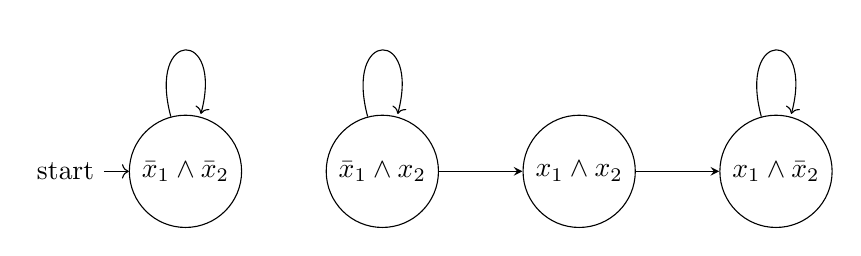
\begin{tikzpicture}[%
scale=0.7,%
trans/.style={->,>=stealth},%
smallnode/.style={inner sep=1.4},%
node distance=2.5cm,%
  ]
    \node[initial, state](1){$\bar x_1 \land \bar x_2$};
    
    \node[state] (2) [right of=1] {$\bar x_1 \land x_2$};
    
    \node[state] (3) [right of=2] {$ x_1 \land x_2$};
    
    \node[state] (4) [right of=3] {$ x_1 \land \bar x_2$};
    
        \draw[trans] (2) to node {} (3);
        
        \draw[trans] (3) to node {} (4);    
   
          \path (1) edge [loop above] node {} (1)
          (2) edge [loop above] node {} (2)
          (4) edge [loop above] node {} (4)

          ;
);
  \end{tikzpicture}
  \caption{Transition Graph of $B$.}
 \end{figure}
 \label{ex1}  


Now given the property $P = \bar x_1 \lor x_2$, we want to check whether the bad state $\bar P = x_1 \land \bar x_2$ is reachable: \\ \par

\textbf{1. Step: Check for 0-Counter-Example} \\ 
We need to make sure that $I \Rightarrow P$, we do that by testing if $I \land \bar P$ is satisfiable: 
\begin{equation*}
\underbrace{\bar x_1 \land \bar x_2}_{I} \land \underbrace{x_1 \land \bar x_2}_{\bar P}
\end{equation*}
Which is unsatisfiable because $\bar x_1 \land x_1$, that means there is no 0-counter-example, we continue by initializing $F_0 = I$\\ \\ \par

\textbf{2. Step: First Transition} \\
Check if $F_0 \land T \Rightarrow P'$ by testing if $F_0 \land T \land \bar P'$ is satisfiable:
\begin{equation*}
\underbrace{\bar x_1 \land \bar x_2}_{F_0} \land \underbrace{( x_1 \lor \bar x_2 \lor x_2') \land (x_1 \lor x_2 \lor \bar x_1') \land (\bar x_1 \lor x_1') \land (\bar x_1 \lor \bar x_2') \land (x_2 \lor \bar x_2')}_{T} \land \underbrace{x_1' \land \bar x_2'}_{\bar P'}
\end{equation*}

Which is unsatisfiable because $\bar x_1 \land \bar x_2 \land (x_1 \lor x_2 \lor x_1') \land \bar x_1'$ is not satisfiable. We generate no proof-obligation and continue with the propagation-phase. \\ \\

\textbf{3. Step: First Propagation-Phase} \\ Initialize the new frame $F_1 = P$ \\
For each clause $c$ in $F_0$ we check $F_0 \land T \land \bar c'$ for unsatisfiability to strengthen $F_1$.
\begin{itemize}
\item $c = \bar x_1:$
\begin{equation*}
\bar x_1 \land \bar x_2 \land T \land x_1'
\end{equation*}
The conjunction is unsatisfiable because $\bar x_1 \land \bar x_2 \land (x_1 \lor x_2 \lor x_1') \land \bar x_1'$ is not satisfiable.\\ We add $\bar x_1$ to $F_1$ resulting in $F_1 = P \land \bar x_1$ \\

\item$c = \bar x_2:$
\begin{equation*}
\bar x_1 \land \bar x_2 \land T \land x_2'
\end{equation*}
The conjunction is unsatisfiable because $\bar x_1 \land \bar x_2 \land (x_2 \lor \bar x_2') \land x_2'$ is not satisfiable. \\ We add $\bar x_2$ to $F_1$ resulting in $F_1 = P \land \bar x_1 \land \bar x_2$
\end{itemize}
That concludes the propagation-phase resulting in the new frame
\begin{equation*}
F_1 =(\bar x_1 \lor x_2) \land \bar x_1 \land \bar x_2
\end{equation*}
and because $F_1 \not\equiv F_0$ we continue. \\ \\ \\

\textbf{4. Step: Second Transition} \\
Check if $F_1 \land T \Rightarrow P'$ by testing if $F_1 \land T \land \bar P'$ is satisfiable: 
\begin{equation*}
(\bar x_1 \lor x_2) \land \bar x_1 \land \bar x_2 \land T \land x_1' \land \bar x_2'
\end{equation*}
Which is unsatisfiable because $\bar x_1 \land \bar x_2 \land (x_1 \lor x_2 \lor \bar x_1') \land x_1'$ is not satisfiable. We again do not generate a proof-obligation, so that we continue with the second propagation-phase. \\ \\ \par

\textbf{5. Step: Second Propagation-Phase} \\
Initialize the new frame $F_2 = P$ \\
We need to check every clause $c$ in $F_1$ if $F_1 \land T \land \bar c'$ is unsatisfiable to strengthen $F_2$.\\ We  skip $P$. 
\begin{itemize}
\item $c = \bar x_1:$
\begin{equation*}
(\bar x_1 \lor x_2) \land \bar x_1 \land \bar x_2 \land T \land x_1'
\end{equation*}
The conjunction is unsatisfiable because $\bar x_1 \land \bar x_2 \land (x_1 \lor x_2 \lor \bar x_1') \land x_1'$ is not satisfiable \\
We add $\bar x_1$ to $F_2$ resulting in
$F_2 = P \land \bar x_1$ \\

\item $c = \bar x_2:$ 
\begin{equation*}
(\bar x_1 \lor x_2) \land \bar x_1 \land \bar x_2 \land T \land x_2'
\end{equation*}
The conjunction is unsatisfiable because $\bar x_2 \land (x_2 \lor \bar x_2') \land x_2'$ is not satisfiable. \\
We add $\bar x_2$ to $F_2$ resulting in
$F_2 = P \land \bar x_1 \land \bar x_2$

\end{itemize}

With no more clauses left the second propagation-phase ends, resulting in 
\begin{equation*}
F_2 = (\bar x_1 \lor x_2) \land \bar x_1 \land \bar x_2 \equiv F_1
\end{equation*}
The algorithm terminates returning that the property always holds and
\begin{equation*}
(\bar x_1 \lor x_2) \land \bar x_1 \land \bar x_2
\end{equation*}
 being an inductive invariant.

\section{Possible Improvements}
In this section we discuss possible improvements to the shown algorithm to make it more efficient. The most time consuming part of the PDR algorithm is the solving of SAT-queries, the larger the query the more time it takes. To improve this there are several ways to keep SAT-queries small.

\subsection{Generalization of States}
Blocking one state at a time is ineffective.  \\
When blocking a state $s$ do not add $\bar s$ but try to find and add a cube $c \subseteq \bar s$. \\
Most modern SAT-solver not only return unsatisfiable but also a reason for it, either by an UNSAT-core or through a final conflict-clause. Both of them deliver information about which clauses were actually used in the proof. To find $c$ just remove unused clauses of $s$.

\subsection{Ternary Simulation}
To reduce proof-obligations it is possible to eliminate not needed state variables by checking a satisfying assignment using ternary simulation. \\
Ternary logic extends the binary logic by introducing a new valuation: $X$, called unknown, and new rules:
\begin{align*}
(X \land false) &= false, \\ (X \land true) &= X, \\ (X \land X) &= X, \\ \bar X &= X
\end{align*}
To remove state variables, set one variable at a time to $X$ and try to transition to a next state using the transition relation, the variable is needed if $X$ propagates into the next state, if it does not remove the variable from the proof-obligation. \\ \\
Reconsider the prior \hyperref[ex2]{example's} first blocking phase resulting in the proof-obligation$(q, 1)$ with bad state $q = x_1 \land \bar x_2 \land \bar x_3$, we now want to reduce that proof-obligation using ternary simulation: \par


First of all, the transition formula:
\begin{equation*}
\underbrace{x_1 \land \bar x_2 \land \bar x_3}_{q} \land \underbrace{(x_1 \lor \bar x_2' ) \land ( \bar x_1 \lor x_2') \land (x_2 \lor \bar x_3') \land ( \bar x_2 \lor x_3')}_{T}
\end{equation*}

Now set $x_1 = X$: \\
\begin{equation*}
\underbrace{X \land \bar x_2 \land \bar x_3}_{q} \land \underbrace{(X \lor \bar x_2' ) \land ( \bar x_1 \lor x_2') \land (x_2 \lor \bar x_3') \land ( \bar x_2 \lor x_3')}_{T}
\end{equation*}
$(X \lor \bar x_2')$ is unknown meaning that $x_1$  is needed. \\ \\

Now set $x_2 = X$: \\
\begin{equation*}
\underbrace{x_1 \land X \land \bar x_3}_{q} \land \underbrace{(x_1 \lor \bar x_2' ) \land ( \bar x_1 \lor x_2') \land (X \lor \bar x_3') \land ( X \lor x_3')}_{T}
\end{equation*}

$(X \lor \bar x_3')$ is unknown meaning that $x_2$  is needed as well. \\ \\

Now set $x_3 = X$: \\
\begin{equation*}
\underbrace{x_1 \land \bar x_2 \land X}_{q} \land \underbrace{(x_1 \lor \bar x_2' ) \land ( \bar x_1 \lor x_2') \land (x_2 \lor \bar x_3') \land ( \bar x_2 \lor x_3')}_{T}
\end{equation*}
Because there is no clause being unknown, $x_3$ can be removed from the proof-obligation. We get the reduced proof-obligation$(x_1 \land \bar x_2, 1)$

\pagebreak


\chapter{PDR for Software} \label{sec3}
After we have seen how PDR works on systems based on propositional logic, we show in this chapter how to extend the approach to work on systems based on first-order logic. We need to \textsl{lift} the approach from bit-level to first-order logic. We base our approach on the technique described by Lange et al ~\cite{DBLP:conf/fmcad/0001NN15}. There are however other ways to accomplish this, see chapter 5 for an overview of other techniques. \par To use PDR on software we first need some new definitions and other preliminaries.

\section{Preliminaries}


The lifted algorithm no longer works on boolean transition systems but on control flow graphs.

A control flow graph (CFG) $\mathcal{A} = (X, L, G, \ell_0, \ell_E)$ is a graph, consisting of: 
\begin{itemize}
\item A finite set of variables $X$
\item A finite set of locations $L$
\item A finite set of transitions $G \subseteq L \times FO \times L$, $FO$ being a quantifier free first-order logic formula over variables in $X$ and $X' = \{x \in X \ | \ x' \in X'\}$
\item An initial location $\ell_0 \in L$
\item  An error location $\ell_E \in L$
\end{itemize}
The lifted algorithm tries to prove whether $\ell_E$ is reachable by finding a feasible path from $\ell_0$ to $\ell_E$. \par

For example consider the CFG $\mathcal{A} = (X, L, G, \ell_0, \ell_E)$ in Figure 3.1, where
\begin{itemize}
\item $X = \{x\}$
\item $L = \{\ell_0, \ell_1, \ell_2, \ell_3, \ell_E\}$
\item $G = \{(\ell_0, x' = 0, \ell_1), (\ell_1, x' = x + 1, \ell_2), (\ell_2, x = 1, \ell_E), (\ell_2, x \neq 1, \ell_3) \} $
\end{itemize}
\pagebreak

\begin{figure}[H]
\centering
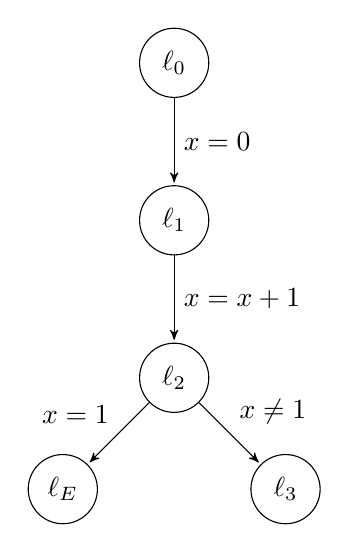
\begin{tikzpicture}[%
    ->,
    >=stealth', shorten >=1pt, auto,
    node distance=2cm, scale=1, 
    transform shape, align=center,    
smallnode/.style={inner sep=1.4}
  ]
    \node[state](1){$\ell_0$};
    
    \node[state] (2) [below of=1] {$\ell_1$};
    
    \node[state] (3) [below of=2] {$\ell_2$};
    
    \node[state] (4) [below right of=3] {$\ell_3$};
    
    \node[state] (5) [below left of=3] {$\ell_E$};
    
    
          \path (1) edge node {$x = 0$} (2)
          (2) edge node {$x = x + 1$} (3)
          (3) edge node {$x \neq 1$} (4)
          (3) edge [edge label={$x = 1$}, swap] node {} (5)
          ;

    
);
  \end{tikzpicture}
  \caption{Graph of $\mathcal{A}$.}
 \end{figure}
 \label{ex7} 

The transition formula $T_{\ell_1 \rightarrow \ell_2}$ from one location $\ell_1$ to another location $\ell_2$ is defined as:
\begin{equation*}
T_{\ell_1 \rightarrow \ell_2} = \begin{cases} (\ell_1, t, \ell_2), & (\ell_1, t, \ell_2) \in G \\
                     false, & otherwise
       \end{cases}
\end{equation*}

Resulting in the global transition formula: \\
$$ T = \bigvee_{(\ell_1, t, \ell_2) \in G} T_{\ell_1 \rightarrow \ell_2}$$

\section{Lifted Algorithm}

To lift our on propositional logic based PDR algorithm to first-order logic we have to modify four aspects of the algorithm:
\begin{itemize}
	
	\item Instead of a global set of Frames $[F_0, ..., F_k]$ we assign each program location $\ell \in L \backslash \{\ell_E\}$ a local set of frames $[F_{0, \ell}, ..., F_{k, \ell}]$. Each frame is now a cube of first-order formulae. As there are now multiple traces, proof-obligations get extended by another parameter, lifted proof-obligations are tuples $(t, \ell, i)$ where $t$ is a first-order formula, $\ell$ describes the location where $t$ has to be blocked, and $i$ is a frame number, called level in the lifted algorithm.
	
	\item 
	Because the states in a CFG are no formulae, the lifted algorithm no longer blocks states but transitions, there are no bad states only bad transitions.
	
	\item Because of the structure of the CFG, it is already known which states lead to the error location, as it is easy to extract the transitions in $G$ that have $\ell_E$ as target, making the next transition phase, that was used to find proof-obligations before, obsolete. \\ If there exists a transition to $\ell_E$ there will be an initial proof-obligation in each iteration of the algorithm, making the blocking-phase no longer optional.
	
	\item The propagation-phase is slimmed, it only checks for termination. In the phase the algorithm checks the frames to find a level $i$ where all locations have a fixpoint, meaning  $F_{i, \ell} = F_{i-1, \ell}$ for every location $\ell \in L \backslash \{l_E \}$, $i$ is called a global fixpoint position. There is no more propagating formulae forward.
\end{itemize}


\begin{figure}[H]
	\begin{algorithm}[H] 
		\begin{algorithmic}[1]
			\Procedure{lifted-PDR-prove}{$L, G$}
			\State check for 0-counter-example
			\State $\ell_0.trace.push(new\ frame(true))$
			\ForAll {$\ell \in L \backslash \{ \ell_0, \ell_E\}$}
			\State $\ell.trace.push(new\ frame(false))$
			\EndFor
			\State $level := 0$
			\Statex
			\Loop
			\ForAll {$\ell \in L \backslash \{\ell_E\}$}
			\State $\ell.trace.push(new\ frame(true))$
			\EndFor
			\State $level:= level + 1$
			\State get initial proof-obligations 
			\Statex
			\While {$\exists$ proof-obligation $(t, \ell, i),$} 
			\State Recursively block proof-obligation
			\If {a proof-obligation$(p, \ell, 0)$ is generated}
			\State{\Return{false}}
			\EndIf
			\EndWhile
			
			\Statex 
			\For {$i = 0;\ i \leq level;\ i:= i + 1$}
			\For {$\ell \in L \backslash \{l_E \}$}
			\If {$\ell.trace[i] \neq \ell.trace[i-1]$}
			\State{break}
			\EndIf
			\EndFor
			\State{\Return{true}}
			\EndFor
			\EndLoop
			\EndProcedure
		\end{algorithmic}
	\end{algorithm}
	\caption{Lifted PDR Algorithm.}
\end{figure}

Figure 3.2 shows the updated PDR algorithm. Given a CFG $\mathcal{A} = (X, L, G, \ell_0, \ell_E)$ we want to check if $\ell_E$ is reachable: \par

Like the bit-level algorithm it starts on line 2 with checking for a 0-counter-example, the algorithm checks whether $\ell_0 = \ell_E$. If so it terminates and returns that $\ell_E$ is indeed reachable, if not it initializes level 0 frames for all locations $\ell \in L \backslash \{\ell_0, \ell_E\}$ as \texttt{false}, and for $\ell_0$ as \texttt{true}. \par
Let $k$ be the current level, so that each location $\ell \in L \backslash \{\ell_E\}$ has frames $[F_{0, \ell}, ..., F_{k, \ell}]$. \\
The algorithm repeats the following phases: \\

\textsl{1. Next Level} \\
In lines 7 to 11, the algorithm initializes for each $\ell \in L \backslash \{\ell_E\}$ a new frame $k + 1$ as \texttt{true}. \\
For each location $\ell \in L$ where $(\ell, t, \ell_E) \in G$ it generates an initial proof-obligation $(t, \ell, k)$. \\


\textsl{2. Blocking-Phase} \\
With the lifted algorithm the blocking-phase is no longer nested in the preceding phase, as we see in line 12 to 15 int he code. Here the algorithm takes proof-obligation $(t, \ell, i)$ with the lowest $i$ and checks for each predecessor location $\ell_{pre}$ if the formula:
\begin{equation*}
F_{i - 1, \ell_{pre}} \land T_{\ell_{pre} \rightarrow \ell} \land t'
\end{equation*}
is satisfiable.
\begin{itemize}
	\item If it is \textsl{satisfiable}, it means that $t$ could not be blocked at $\ell$ on level $i$, the algorithm generates a new proof-obligation $(p, \ell_{pre}, i-1)$ where $p$ is the weakest precondition of $t$ with regard to $T_{\ell_{pre} \rightarrow \ell}$.
	\item If the formula is \textsl{unsatisfiable}, the algorithm strengthens each frame $F_{j, \ell}$, $j \leq i$ with $\bar t$, meaning $F_{j, \ell} = F_{j, \ell} \land \bar t$, blocking $t$ at $\ell$ on level $i$.
\end{itemize}

This continues recursively until either a proof-obligation $(d, \ell, 0)$ is generated, proving that there exists a feasible path to $\ell_E$ terminating the algorithm, or there is no unblocked proof-obligation left. \\

\textsl{3. Propagation-Phase} \\
In lines 16 to 20 the algorithm checks the frames if there exists a global fixpoint position $i$ where
\begin{equation*}
F_{i-1, \ell} = F_{i, \ell}
\end{equation*}
for every location $\ell \in L \backslash \{l_E \}$. \\
If there is such an $i$ the algorithm terminates returning that $\ell_E$ is not reachable. \\ \\


\hspace*{5cm}



\pagebreak

\section{Example}
In this section we show an application of the lifted algorithm on two cases, one where the error state is reachable, and one where it is not.
\subsection{Case 1: Error State is Reachable}
To show an application of the lifted algorithm consider again the example in \hyperref[ex7]{Figure 3.1}, we have CFG  $\mathcal{A} = (X, L, G, \ell_0, \ell_E)$, where
\begin{itemize}
\item $X = \{x\}$
\item $L = \{\ell_0, \ell_1, \ell_2, \ell_3, \ell_E\}$
\item $G = \{(\ell_0, x' = 0, \ell_1), (\ell_1, x' = x + 1, \ell_2), (\ell_2, x = 1, \ell_E), (\ell_2, x \neq 1, \ell_3) \}$
\end{itemize}

We now want to verify whether $\ell_E$ is reachable using the lifted algorithm: \\ \\

\textbf{1. Step: Check for 0-Counter-Example} \\
Is $\ell_0 = \ell_E$?  \\
No, we continue with initializing level 0 by adding to each $\ell \in L \backslash \{\ell_0, \ell_E\}$ a new frame $F_{0, \ell} = false$, for $\ell_0$ adding $F_{0, \ell_0} = true$: \\ \\

\setlength\tabcolsep{0.35em}
\begin{center}
\begin{tabu}{cc}
\toprule
             & level \\
\cmidrule(lr){2-2}
location & 0 \\
\cmidrule{1-2}
$\ell_0$ & $true$ \\
$\ell_1$ & $false$ \\
$\ell_2$ & $false$ \\ 
$\ell_3$ & $false$ \\
\bottomrule
\end{tabu}
\end{center}

\hspace*{5cm}

\textbf{2. Step: Next Level} \\
We initialize new frames for level 1 as \texttt{true}: \\

\begin{center}
\begin{tabu}{ccc}
\toprule
             & \multicolumn{2}{c}{level} \\
\cmidrule(lr){2-3}
location & 0 & 1 \\
\cmidrule{1-3}
$\ell_0$ & $true$ & $true$ \\
$\ell_1$ & $false$ & $true$ \\
$\ell_2$ & $false$ & $true$ \\
$\ell_3$ & $false$ & $true$ \\
\bottomrule
\end{tabu}
\end{center}

\hspace*{3cm}

To generate the initial proof-obligations, we check $G$ and take the transitions where $\ell_E$ is the target. \\ We see, there is one transition $(\ell_2, x = 1, \ell_E)$, that means we have to block $x = 1$ at $\ell_2$ on level 1, resulting in the initial proof-obligation $(x = 1, \ell_2, 1).$ \\ \\ \par

\textbf{3. Step: First Blocking Phase} \\
We need to block the initial proof-obligation $(x = 1, \ell_2, 1)$. Let $\ell_{pre}$ be a predecessor of $\ell_2$, we need to check the formula:
\begin{equation*}
F_{0, l_{pre}} \land T_{\ell_{pre} \rightarrow \ell_2} \land x' = 1
\end{equation*}
for satisfiability. As there is only one predecessor $\ell_1$ we check:
\begin{equation*}
\underbrace{false}_{F_{0, \ell_1}} \land \underbrace{x' = x + 1}_{T_{\ell_1 \rightarrow \ell_2}} \land x' = 1
\end{equation*}

Which is unsatisfiable \\
We add $\overline{(x=1)} \equiv x \neq 1$ to $F_{0, \ell_2}$ and $F_{1, \ell_2}$, blocking $x=1$ at $\ell_2$ on level 1. \\

\begin{center}
\begin{tabu}{ccc}
\toprule
             & \multicolumn{2}{c}{level} \\
\cmidrule(lr){2-3}
location & 0 & 1 \\
\cmidrule{1-3}
$\ell_0$ & $true$ & $true$ \\
$\ell_1$ & $false$ & $true$ \\
$\ell_2$ & $false \land x \neq 1$ & $true \land x \neq 1$ \\
$\ell_3$ & $false$ & $true$ \\
\bottomrule
\end{tabu}
\end{center}

\hspace*{3cm}


Because there are no proof-obligations left we continue with the propagation-phase. \\ \\ \par

\textbf{4. Step: First Propagation-Phase} \\
Check if there exists a global fixpoint position $i$ where
\begin{equation*}
F_{i-1, \ell} = F_{i, \ell}
\end{equation*}
for every location $\ell \in L \backslash \{l_E \}$. \\
We see there is no such $i$, we continue with the next level. \\ \\ \par


\textbf{5. Step: Next Level} \\
We initialize new frames for level 2 as \texttt{true}: \\

\begin{center}
\begin{tabu}{cccc}
\toprule
             & \multicolumn{3}{c}{level} \\
\cmidrule(lr){2-4}
location & 0 & 1 & 2 \\
\cmidrule{1-4}
$\ell_0$ & $true$ & $true$ & $true$ \\
$\ell_1$ & $false$ & $true$ & $true$ \\
$\ell_2$ & $false \land x \neq 1$ & $true \land x \neq 1$ & $true$ \\
$\ell_3$ & $false$ & $true$ & $true$ \\
\bottomrule\end{tabu}
\end{center}

\hspace*{3cm}


Again generate the initial proof-obligation which is the same as before but on level 2 now, we have initial proof-obligation $(x = 1, \ell_2, 2)$ \\ \\ \par

\textbf{6. Step: Second-Blocking Phase} \\
We need to block the proof-obligation $(x = 1, \ell_2, 2)$ by checking
\begin{equation*}
\underbrace{true}_{F_{1, \ell_1}} \land \underbrace{x' = x + 1}_ {T_{\ell_1 \rightarrow \ell_2}} \land x' = 1
\end{equation*}
for satisfiability. Which is satisfiable with $ p = (x = 0)$. Because $p$ being also the weakest precondition, we generate a new proof-obligation $(p, \ell_1, 1)$, meaning we need to block $p$ at location $\ell_1$ on level 1. \par
Take the new proof-obligation $(x=0, \ell_1, 1)$ and check 
\begin{equation*}
\underbrace{true}_{F_{0, \ell_0}} \land \underbrace{x' = 0}_ {T_{\ell_{0} \rightarrow \ell_1}} \land \underbrace{x' = 0}_{p'}
\end{equation*}
for satisfiability. \\
Which is valid, with \texttt{true} being the weakest precondition, we generate the new proof-obligation $(true, l_0, 0)$ and because this obligation is on level 0 we terminate, stating that $\ell_E$ is reachable by the counter-example trace:
\begin{equation*}
\ell_0 \rightarrow \ell_1 \rightarrow \ell_2 \rightarrow \ell_E
\end{equation*}


\pagebreak

\subsection{Case 2: Error State is Unreachable}
Figure 3.3 shows an CFG $\mathcal{B} = (X, L, G, \ell_0, \ell_E)$ with reachable error state, where
\begin{itemize}
\item $X = \{x, y\}$
\item $L = \{\ell_0, \ell_1, \ell_2, \ell_E\}$
\item $G = \{(\ell_0, x' = 0 \land y' = x', \ell_1), (\ell_1, x' = x+1 \land y' = y+1, \ell_1),\\ (\ell_1, x = y, \ell_2), (\ell_1, x \neq y, \ell_E) \}$
\end{itemize}



\begin{figure}[H]
\centering
\hspace*{3cm}
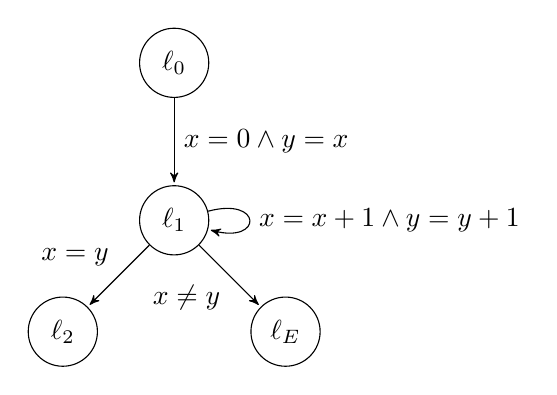
\begin{tikzpicture}[%
    ->,
    >=stealth', shorten >=1pt, auto,
    node distance=2cm, scale=1, 
    transform shape, align=center,    
smallnode/.style={inner sep=1.4}
  ]
    \node [state](1){$\ell_0$};
    
    \node[state] (2) [below of=1] {$\ell_1$};
    
    \node[state] (3) [below left of=2] {$\ell_2$};
    
    \node[state] (4) [below right of=2] {$\ell_E$};
    
    
    
          \path (1) edge node {$x = 0 \land y = x$} (2)
          (2) edge [loop right] node {$x = x + 1 \land y = y + 1$} (2)
          (2) edge [edge label={$x = y$}, swap] node {} (3)
          (2) edge [edge label={$x \neq y$}, swap] node {} (4)
          ;

    
);
  \end{tikzpicture}
  \caption{Graph of $\mathcal{B}$.}
 \end{figure}
 \label{ex1} 

We now want to check whether $\ell_E$ is reachable, using the lifted algorithm: \par

\textbf{1. Step: Check for 0-Counter-Example} \\
Is $\ell_0 = \ell_E$? \\
No, we continue with initializing level 0 by adding to each $\ell \in L \backslash \{\ell_0, \ell_E\}$ a new frame $F_{0, \ell} = false$, for $\ell_0$ adding $F_{0, \ell_0} = true$. \\ \\


\setlength\tabcolsep{0.35em}
\begin{center}
\begin{tabu}{cc}
\toprule
             & level \\
\cmidrule(lr){2-2}
location & 0 \\
\cmidrule{1-2}
$\ell_0$ & $true$ \\
$\ell_1$ & $false$ \\
$\ell_2$ & $false$ \\
\bottomrule
\end{tabu}
\end{center}

\hspace*{5cm}


\textbf{2. Step: Next Level} \\
We initialize new frames for level 1 as \texttt{true}: \\

\begin{center}
\begin{tabu}{ccc}
\toprule
             & \multicolumn{2}{c}{level} \\ 
\cmidrule(lr){2-3}
location & 0 & 1 \\
\cmidrule{1-3}
$\ell_0$ & $true$ & $true$ \\
$\ell_1$ & $false$ & $true$ \\
$\ell_2$ & $false$ & $true$ \\
\bottomrule
\end{tabu}
\end{center}

\hspace*{5cm}


We see there is only one transition leading to $\ell_E$, $(\ell_1, x \neq y, \ell_E)$. We get the initial proof-obligation $(x \neq y, \ell_1, 1)$. \\ \\ \par
\textbf{3. Step: First Blocking Phase} \\
To block the initial proof-obligation $(x \neq y, \ell_1, 1)$ we check each predecessor of $\ell_1$:

\begin{itemize}
\item predecessor: $\ell_0$
\begin{equation*}
\underbrace{true}_{F_{0, \ell_0}} \land \underbrace{x' = 0 \land y' = x'}_{T_{\ell_0 \rightarrow \ell_1}} \land  x' \neq y'
\end{equation*}
Which is unsatisfiable, we add $\overline{(x \neq y)} \equiv x = y$ to $F_{0, \ell_1}$ and $F_{1, \ell_1}$: \\

\begin{center}
\begin{tabu}{ccc}
\toprule
             & \multicolumn{2}{c}{level} \\
\cmidrule(lr){2-3}
location & 0 & 1 \\
\cmidrule{1-3}
$\ell_0$ & $true$ & $true$ \\
$\ell_1$ & $false \land x = y$ & $true \land x = y$ \\
$\ell_2$ & $false$ & $true$ \\
\bottomrule
\end{tabu}
\end{center}

\hspace*{5cm}

\item predecessor: $\ell_1$
\begin{equation*}
\underbrace{false \land x = y}_{F_{0, \ell_1}} \land \underbrace{x' = x + 1 \land y' = y + 1'}_{T_{\ell_1 \rightarrow \ell_1}} \land  x' \neq y'
\end{equation*}
Which is unsatisfiable as well, but because $x = y$ has already been added to $F_{0, \ell_1}$ and $F_{1, \ell_1}$ we move on.

\end{itemize}
 As there are no proof-obligations left, we continue with the first propagation-phase. \\ \\ \par
 
\textbf{4. Step: First Propagation-Phase} \\
Check if there exists a global fixpoint position $i$ where
\begin{equation*}
F_{i-1, \ell} = F_{i, \ell}
\end{equation*}
for every location $\ell \in L \backslash \{l_E \}$. \\
We see there is no such $i$, we continue with the next level. \\ \\ \par

\textbf{5. Step: Next Level} \\
We initialize new frames for level 2 as \texttt{true}: \\

\begin{center}
\begin{tabu}{cccc}
\toprule
             & \multicolumn{3}{c}{level} \\
\cmidrule(lr){2-4}
location & 0 & 1 & 2\\
\cmidrule{1-4}
$\ell_0$ & $true$ & $true$ & $true$ \\
$\ell_1$ & $false \land x = y$ & $true \land x = y$ & $true$\\
$\ell_2$ & $false$ & $true$ & $true$ \\
\bottomrule
\end{tabu}
\end{center}

\hspace*{5cm}

Again we generate the initial proof-obligation which is the same as before but on level 2 now, we have the initial proof-obligation $(x \neq y, \ell_1, 2).$ \\ \\ \par


\textbf{6. Step: Second Blocking Phase} \\
To block proof-obligation $(x \neq y, \ell_1, 2)$ we check the predecessors of $\ell_1$:

\begin{itemize}
\item predecessor: $\ell_0$
\begin{equation*}
\underbrace{true}_{F_{1, \ell_0}} \land \underbrace{x' = 0 \land y' = x'}_{T_{\ell_0 \rightarrow \ell_1}} \land  x' \neq y'
\end{equation*}
Which is unsatisfiable, we add $\overline{(x \neq y)} \equiv x = y$ to $F_{0, \ell_1}$, $F_{1, \ell_1}$ and $F_{2, \ell_1}$:

\begin{center}
\begin{tabu}{cccc}
\toprule
             & \multicolumn{3}{c}{level} \\
\cmidrule(lr){2-4}
location & 0 & 1 & 2\\
\cmidrule{1-4}
$\ell_0$ & $true$ & $true$ & $true$ \\
$\ell_1$ & $false \land x = y$ & $true \land x = y$ & $true \land x = y$ \\
$\ell_2$ & $false$ & $true$ & $true$ \\
\bottomrule
\end{tabu}
\end{center}

\hspace*{5cm}

\item predecessor: $\ell_1$
\begin{equation*}
\underbrace{true \land x = y}_{F_{1, \ell_1}} \land \underbrace{x' = x + 1 \land y' = y + 1}_{T_{\ell_1 \rightarrow \ell_1}} \land  x' \neq y'
\end{equation*}
Which is unsatisfiable as well, but because $x = y$ has already been added to $F_{0, \ell_1}$, $F_{1, \ell_1}$, and $F_{2, \ell_1}$ we move on.
\end{itemize}

As there are no proof-obligations left, we continue with the second propagation-phase \\ \\ \par

\textbf{7. Step: Second Propagation-Phase} \\

\begin{center}
\begin{tabu}{cccc}
\toprule
             & \multicolumn{3}{c}{level} \\
\cmidrule(lr){2-4}
location & 0 & 1 & 2\\
\cmidrule{1-4}
$\ell_0$ & $true$ & $true$ & $true$ \\
$\ell_1$ & $false \land x = y$ & $true \land x = y$ & $true \land x = y$ \\
$\ell_2$ & $false$ & $true$ & $true$ \\
\bottomrule
 \multicolumn{1}{c}{} &  \multicolumn{1}{c}{} & \multicolumn{2}{c}{\upbracefill} \\[-1ex]
 \multicolumn{1}{c}{} & \multicolumn{1}{c}{} & \multicolumn{2}{c}{$\scriptstyle global\ fixpoint$}\\
\end{tabu}
\end{center}

\hspace*{5cm}

We see that level 1 equals level 2 on all locations, with that we found global fixpoint position $i = 2$, the forumulas at that position are the inductive invariants proving that $\ell_E$ is not reachable.


\section{Possible Improvements}
\label{improvements}

As shown before, lifting PDR from bit-level to control flow graphs is possible. The problem of large, time consuming queries to the solver remain however. Is it possible to lift the improvements of the bit-level algorithm too? \par

\textsl{Ternary Simulation} cannot be used on first-order formulae, because as we have seen in section 2.4.2 ternary simulation extends the binary propositional logic by a third value and checks whether that value propagates through formulae. First-order logic is not binary, extending its value space would not work the way it does on propositional logic,
making it impossible to use to reduce lifted proof-obligations. \par
In the following we present techniques to improve our base algorithm.
\subsection{Syntactical Analysis}
It is possible to remove a cube $c$ from a proof-obligation if no variable in $c$ is assigned in $T$, and either $c$ is already contained in a frame or there is an \texttt{assume $c$} transition in $T$. Making the obligation more general.


\subsection{Weakest Precondition}
The definition of the lifted algorithm above already contains an improvement, using weakest preconditions to overapproximate predecessor states. Without weakest preconditions we would have to generate a new explicit proof-obligation for each possible predecessor state. Now we have one proof-obligation containing every possible predecessor.


\subsection{Disjunctive Normal Form}
It is possible to transform cubes into clauses by simply negating them. When there is a large proof-obligation we can use this to generate the disjunctive normal form and split the large obligation into smaller ones by taking each cube in the disjunctive normal form as a new proof-obligation, saving time because smaller queries are solved faster.

\subsection{Interpolation}
Adding the negated proof-obligation to the frames works well in most cases. Consider Figure 3.4, we see a simple program with a loop. The initial proof-obligation on level $i$ is $(x = 1, \ell_1, i)$, because $\ell_1$ has two predecessors we have to check:
\begin{equation}
	F_{\ell_1, i - 1} \land x' = x + 1 \land x' = 1
\end{equation}
\begin{equation}
F_{\ell_0, i - 1} \land x' = 2 \land x' = 1
\end{equation}
for satisfiability. \\
Formula (3.1) is satisfiable until we get a proof-obligation on level 1, because frame $F_{\ell_1, 0}$ is always false. \\
Formula (3.2) is always unsatisfiable, in each level we add $x \neq 1$ to $\ell_1$'s frames. That formula however is not strong enough to block the chain of satisfiable obligations of (3.1) in the next level, which is inefficient.

\begin{figure}[H]
	\centering
	\hspace*{3cm}
	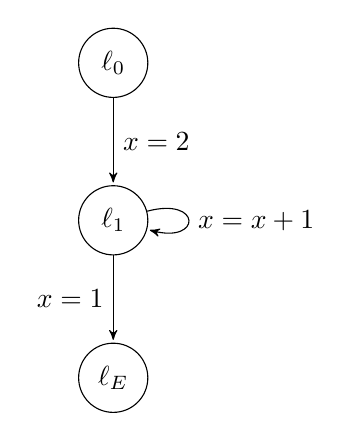
\begin{tikzpicture}[%
	->,
	>=stealth', shorten >=1pt, auto,
	node distance=2cm, scale=1, 
	transform shape, align=center,    
	smallnode/.style={inner sep=1.4}
	]
	\node[state](1){$\ell_0$};
	
	\node[state] (2) [below of=1] {$\ell_1$};
	
	\node[state] (3) [below of=2] {$\ell_E$};
	
	
	
	
	\path (1) edge node {$x = 2$} (2)
	(2) edge [loop right] node {$x = x + 1$} (2)
	(2) edge [edge label={$x = 1$}, swap] node {} (3)
	;
	
	
	);
	\end{tikzpicture}
	\caption{Simple Program.}
\end{figure}
\label{exInterpol} 

Instead, consider using interpolants.
Let $(A, B)$ be a pair of formulae such that $A \land B$ is unsatisfiable. An interpolant $I$ for $(A, B)$ is a formula fulfilling the following characteristics:
\begin{itemize}
	\item $A \Rightarrow I$
	\item $I \land B$ is unsatisfiable
	\item $I$ consists only of variables found in $A \cap B$
\end{itemize}
\par
Now, an interpolant for the unsatisfiable formula (3.2) would be $x = 2$, if we add that to $\ell_1$'s frames, we would be able to block formula (3.1) much earlier. \\



\pagebreak


\chapter{PDR in \textsc{Ultimate}}
In this chapter we introduce the program analysis framework \textsc{Ultimate} \footnote{https://github.com/ultimate-pa}, and its tool \textsc{Ultimate Automizer}, we will show how we integrated PDR, and detail which improvements were considered.
\section{Introduction \textsc{Ultimate}}
\textsc{Ultimate} is a program analysis framework, based on \textsl{plugins} that can be executed one after another to form \textsl{toolchains} which can perform various tasks. An advantage of this modularity is that it is relatively easy to implement new toolchains as a lot of plugins can be reused creating much less overhead. There are five types of plugins: 
\begin{itemize}
\item Source plugins define a file-to-model transformation

\item  Analyzer plugins take a model as input and modifies it

\item Generator plugins have a similar functionality as Analyzer plugins but they can additionally produce new models

\item Output plugins do not produce or modify anything, they write models into files

\item The last plugin cannot be used in toolchains per say, they act more like a library providing additional functionality to other plugins

\end{itemize}

\section{Implementation}
To implement PDR in \textsc{Ultimate} we chose to implement a new library plugin \textsl{Library-PDR}, that will be executed as part of \textsc{Ultimate Automizer} \cite{Heizmann:2013:SMC:2526861.2526864}. \par 
\textsc{Ultimate Automizer} (\textsc{Automizer} in the following) is a software verifier that is capable of checking safety and liveness properties. It uses an automata-based \cite{DBLP:conf/cav/HeizmannHP13} instance of the CEGAR scheme, that works like this: \\

\textsl{1. Get an Error Trace:}
In each new iteration choose a sequence of statements, called trace, that start at the initial location and lead to an error location. Check whether the trace is feasible or infeasible.
 \begin{itemize}
	\item If the trace is \textsl{feasible} then the program is proven unsafe, meaning there exists a possible program execution leading to an error location.
	\item If the trace is \textsl{infeasible}, calculate a proof for the infeasibility by computing a sequence of predicates along the trace, called sequence of interpolants. Then, in a following refinement step, try to eliminate every other trace that can be proven infeasible using that sequence of interpolants, these traces are then being subtracted from the set of potentially error traces.
 \end{itemize}

\textsl{2. Check Feasability:}
To check a trace for feasibility we use our newly integrated Library-PDR. \par
 A path-program is
 
 The sequence of interpolants are the entries in the frames on the global fixpoint.
 

\section{Improvements}
As we have seen in \hyperref[improvements]{Section 4.4} there are a plethora of possible ways to make PDR more efficient. In this section we present implemented improvements to our approach.
\subsection{Caching of Proof-Obligation Queue}
We always start each new level with the initial proof-obligation, and generate a chain of proof-obligations, until the most recent one is blocked. We then recursively block all predecessor obligations, adding new information to the frames. This chain of obligations does not change, once a new obligation is generated it needs to be blocked in each successive level.\\
Now as a result of the backwards search nature of PDR, each new level has to create that chain of proof-obligations from the beginning again. That results in a lot of overhead because we have to calculate the same chain of obligations times and times again. \par
%For example, let $i$ be the current level, we have seen and blocked the initial proof-obligation $i$ times, its successor obligation $i-1$ times and so on. \par
Our idea was to cache the proof-obligation queue and always start a new level with the latest generated one, so we save the process of generating already known obligations. \par For that we introduced a \textsl{global level} variable serving as the level counter, and changed the levels of each proof-obligation to be \textsl{subtracted} from the global level, resulting in a relative level = $global\ level - local\ level$, with that every proof-obligation is at its corresponding level of generation. \par For example, the initial proof-obligation has its local level 0, so that $relative\ level = global\ level - 0 = global\ level$, because the initial obligation always is on the global level, take an obligation that we generate from the initial one, it has local level 1 so that relative level = global level - 1 means that this proof-obligation comes immediately after the initial one. \par
Something that cannot be saved is blocking of the previous proof-obligation chain. We can only ignore the chain of proof-obligations leading to the newest one. The chain of blocking the ones before up to the initial obligation is necessary, because otherwise the frames are not updated properly.
In Figure 4.1 we see a representation of both chains of proof-obligation where the chain leading down the most recent one is highlighted, signaling that this chain can be skipped.

\begin{figure}[H]
\centering
\resizebox{\textwidth}{!}{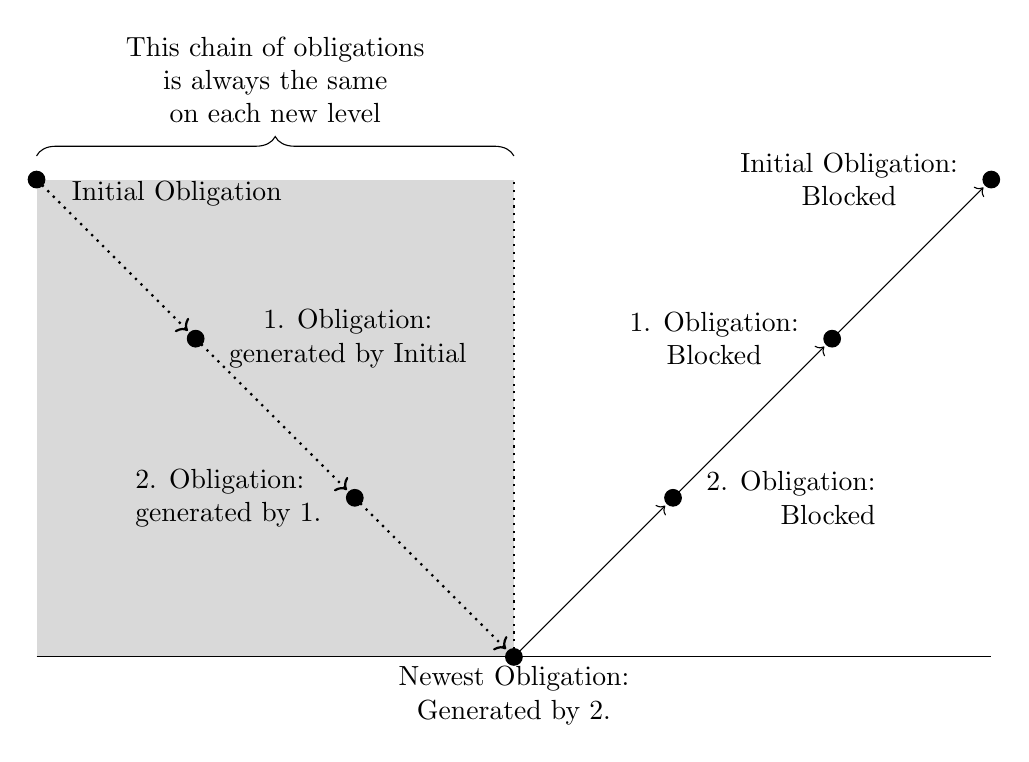
\begin{tikzpicture}[decoration={brace,mirror,amplitude=7}]


\fill[black!15!white] (0,0) -- (0,\textwidth/2) -- (\textwidth/2,\textwidth/2) -- (\textwidth/2, 0) -- cycle;

% horizontal axis
\draw[-] (0,0) -- (\textwidth,0) node[below=3mm] {};


%1.
\filldraw (0,\textwidth/2) circle (3pt) node[align=right, below right, label={[xshift=2mm, yshift=1mm, below right]Initial Obligation}] {};

%connection 1. and 2.
\draw [thick, dotted, ->]
(0,\textwidth/2) --(\textwidth/6 - 1mm,\textwidth/3 + 1mm);

%2.
\filldraw (\textwidth/6,\textwidth/3) circle (3pt) node[align=center,   right=3mm] {1. Obligation: \\ generated by Initial};

%connection 2. and 3.
\draw [thick, dotted, ->]
(\textwidth/6,\textwidth/3) --(\textwidth/3 - 1mm,\textwidth/6 + 1mm);

%3.
\filldraw (\textwidth/3,\textwidth/6) circle (3pt) node[align=left,   left=3mm] {2. Obligation: \\ generated by 1.};

%connection 3. and 4.
\draw [thick, dotted, ->]
(\textwidth/3,\textwidth/6) --(\textwidth/2 - 1mm,0 + 1mm);

%4.
\filldraw (\textwidth/2,0) circle (3pt) node[align=center,   below] {Newest Obligation: \\ Generated by 2.};

%4 and 3'
\draw [->]
(\textwidth/2,0 ) -- (\textwidth - \textwidth/3 - 1mm,\textwidth/6 - 1mm);

%3.'
\filldraw (\textwidth - \textwidth/3,\textwidth/6) circle (3pt) node[align=right,   right=3mm] {2. Obligation: \\ Blocked};


%3' and 2'
\draw [->]
(\textwidth - \textwidth/3, \textwidth/6 ) -- (\textwidth - \textwidth/6 - 1mm,\textwidth/3 - 1mm);


%2.'
\filldraw (\textwidth - \textwidth/6,\textwidth/3) circle (3pt) node[align=center, left=3mm] {1. Obligation: \\ Blocked};


%connection 2.' and 1.'
\draw [->]
(\textwidth - \textwidth/6,\textwidth/3) -- (\textwidth - 1mm,\textwidth/2 - 1mm);


%1.'
\filldraw (\textwidth,\textwidth/2) circle (3pt) node[align=center,   left=3mm] {Initial Obligation: \\ Blocked};


% ranges
%\draw	(1,3.5) node{{\scriptsize Constant flux}};
%		(4,3.5) node{{\scriptsize Field weakening}};

\draw[thick, dotted] (\textwidth/2,0) -- (\textwidth/2,\textwidth/2) node[] {};



% Vertical axis
%\draw[] (0,0) -- (0,\textwidth/2) node[left=5mm] {};
% \draw[] (\textwidth,0) -- (\textwidth,\textwidth/2) node[left=5mm] {};

\draw [decorate] (\textwidth/2, \textwidth/2 + 3mm) -- node[above=3mm, align=center]{This chain of obligations \\ is always the same \\ on each new level} (0, \textwidth/2 + 3mm);

\end{tikzpicture}}
\caption{Chain of Proof-Obligation Generation.}
\label{fig:the_nice_figure}
\end{figure}
 

\subsection{Ignoring Already Blocked Proof-Obligations}
Besides changing the levels of proof-obligations to be relative, we also expanded the proof-obligations with a list of already seen and blocked SMT-solver queries. \par Before we consider a new call to the SMT-solver we first check the given query whether it has already been proven unsatisfiable, if so, we consider the obligation blocked and add the negated formula to the frames, if we prove an unknown query as unsatisfiable we add them to the list of blocked queries. \par
With this memoization we save unnecessary calls to the SMT-solver and with that, time on programs with a lot of identical proof-obligations, in loops for example.

\subsection{Using Preconditions}
As discussed in section 3.4, using weakest preconditions is a really useful addition to the way proof-obligations are generated. \par
We implemented the usage of weakest preconditions in terms of formulas, but were met with problems regarding \texttt{assume}-transitions: \\
Let $\varphi$ and $\psi$ be first-order formulae and $wp$ be the weakest precondition function, we have: 
\begin{equation*}
	wp(\varphi, \texttt{assume}\ \psi) = (\psi \Rightarrow \varphi)
\end{equation*}

Consider the CFG thath contains an \texttt{assume} transition in Figure 4.2. We want to prove if $\ell_E$ is reachable. \\

\begin{figure}[H]
	\centering
	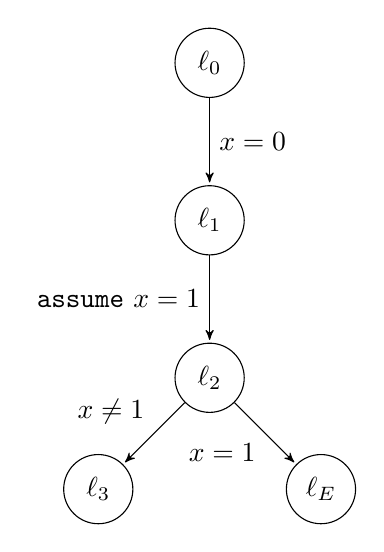
\begin{tikzpicture}[%
	->,
	>=stealth', shorten >=1pt, auto,
	node distance=2cm, scale=1, 
	transform shape, align=center,    
	smallnode/.style={inner sep=1.4}
	]
	\node[state](1){$\ell_0$};
	
	\node[state] (2) [below of=1] {$\ell_1$};
	
	\node[state] (new) [below of=2] {$\ell_2$};
	
	\node[state] (3) [below left of=new] {$\ell_3$};
	
	\node[state] (4) [below right of=new] {$\ell_E$};
	
	
	
	\path (1) edge node {$x = 0$} (2)
	(2) edge [edge label={\texttt{assume} $x=1$}, swap] node {} (new)
	(new) edge [edge label={$x \neq 1$}, swap] node {} (3)
	(new) edge [edge label={$x = 1$}, swap] node {} (4)
	;
	);
	\end{tikzpicture}
	\caption{CFG with \texttt{assume}.}
\end{figure}
\label{assumeEx}

We omit the first iteration of the algorithm and start on level 2 with the initial proof-obligation $(x = 0, \ell_2, 2)$, we check the following formula for satisfiability: 
\begin{equation*}
	true\land \texttt{assume}\ x = 1 \land x' = 1
\end{equation*}

Which is satisfiable, we calculate 
\begin{equation}
	wp(x' = 1, \texttt{assume}\ x = 1) = ((x = 1) \Rightarrow (x' = 1)) 
\end{equation}
\label{wpEx}

Because \texttt{assume} does not change $x$, it becomes apparent that $x' = x$, resulting in 
\begin{equation*}
	((x = 1) \Rightarrow (x = 1)) = true
\end{equation*}
We get the new proof-obligation $(true, \ell_1, 1)$. \\

To block $(true, \ell_1, 1)$, we check the following formula for satisfiability: 
\begin{equation*}
	true\land x' = 0 \land true
\end{equation*}
which is satisfiable as well, we would create a proof-obligation on level 0 and with that would terminate, resulting in the wrong assumption that $\ell_E$ is reachable. \par

To fix this problem we do not use the weakest precondition but just the precondition, which is characterized like this: \\
Let $\varphi$ and $\psi$ be first-order formulae and $pre$ be the precondition function, we have: 
\begin{equation*}
pre(\varphi, \texttt{assume}\ \psi) = (\varphi \land \psi)
\end{equation*}
Now reconsider formula \eqref{wpEx}, to get the new proof-obligation we use the \textsl{pre} function: 
\begin{equation*}
		pre(x' = 1, \texttt{assume}\ x = 1) = ((x = 1) \land (x' = 1))
\end{equation*}
Because $x = x'$ this can be simplified to $x = 1$. We get the new proof-obligation $(x = 1, \ell_1, 1)$.
To block $(x = 1, \ell_1, 1)$, we check the following formula for satisfiability: 
\begin{equation*}
true\land x' = 0 \land x' = 1
\end{equation*}
which is unsatisfiable, and with that we have solved the issue and can continue working on the program. \par


\chapter{Evaluation}
In this chapter we evaluate our implementation and compare it to \textsc{Ultimate}'s Nested Interpolants. \\
We benchmarked PDR with two different SMT-solvers: 
\begin{itemize}
\item SMTInterpol \cite{Zitat03}
\item Z3 \cite{Zitat04}
\end{itemize}
The difference between those is that SMTIterpol interpolates better and is integrated into \textsc{Ultimate}, but on the other hand cannot deal with quantors and non-linear queries. We focus mainly on SMTInterpol.

\section{Comparison}
We used a testing set containing 250 programs.
\begin{figure}[H]
\begin{minipage}[t]{0.5\textwidth}
	\hspace*{-1.5cm}
	\subcaptionbox{CPU Time Comparison.} {
\begin{tikzpicture} 
\begin{axis}[%
width=\textwidth, 
height=\textwidth, 
axis x line=center,
axis y line=center,
x label style={at={(axis description cs:0.5,-0.1)},anchor=north},
y label style={at={(axis description cs:-0.1,.5)},rotate=90,anchor=south},
xtick={0, 5, ..., 170},
ytick={0, 5, ..., 170},
xlabel={PDR SMTInterpol},
ylabel={Nested Interpolants},
xmin=0,
xmax=50,
ymin=0,
ymax=50,
scaled y ticks = false 
]

] 

\addplot [dotted, mark=none,domain=0:100] {x};

\addplot[scatter,only marks]
 table [y = cpu time, x = cpu time pdr, col sep=semicolon, /pgf/number format/read comma as period]  {EvalData/TableAndDifWithoutZ3AndWithoutDupesOnlyFinished.csv}; 

\end{axis} 
\end{tikzpicture}  }
\end{minipage}
 \hfill%
\begin{minipage}[t]{0.5\textwidth}
	\hspace*{-1cm}
	  \subcaptionbox{Memory Usage Comparison.}{
	\begin{tikzpicture} 
	\begin{axis}[%
	width=\textwidth, 
	height=\textwidth, 
	axis x line=center,
	axis y line=center,
	x label style={at={(axis description cs:0.5,-0.1)},anchor=north},
	y label style={at={(axis description cs:-0.25,.5)},rotate=90,anchor=south},
	%xtick={0, 1 * 10^8},
	%ytick={0, 10000000, ..., 350000000},
	xlabel={PDR SMTInterpol},
	ylabel={Nested Interpolants},
	xmin=0,
	xmax=350000000,
	ymin=0,
	ymax=350000000,
	scaled y ticks = false,
	scaled x ticks = false 
	]
	
	] 
	
	\addplot [dotted, mark=none,domain=0:350000000] {x};
	
	\addplot[scatter,only marks]
	table [y = memUsage, x = memUsage PDR, col sep=semicolon]  {EvalData/TableAndDifWithoutZ3AndWithoutDupesMemSpace.csv}; 
	
	\end{axis} 
	\end{tikzpicture} }
\end{minipage}
\caption{Statistics collected from successful benchmarks.}
\end{figure}


\vspace{2cm}

\begin{figure}[H]
\begin{center}
	\begin{tabu}{ccc}
		\cmidrule(lr){2-3}
		Technique & Tests Solved & Solve Time\\
		\cmidrule{1-3}
		Nested Interpolants & 165/250 & 3508s \\
		PDR SMTInterpol& 35/250  & 496s \\
		PDR Z3 & 62/250& 1322s\\
		\bottomrule
	\end{tabu}
\end{center}
\caption{Evaluation Results.}
\end{figure}

\section{Discussion}
In Figure 5.1 we can see that the most benchmark results were equally fast for both techniques, there are however some programs where PDR was significantly slower than the Nested Interpolants. This stems from loops, because Library-PDR does not yet use interpolants, we have trouble solving programs that contain loops, as we have to disprove every single loop iteration, making verification very time consuming. \\
We can see that PDR was in some occasions faster than Nested Interpolants.
Both techniques were more or less on par regarding memory consumption. \par
In Figure 5.2 we see that PDR generally only solved $\frac{1}{7}$ of the benchmarks using SMTInterpol and $\frac{1}{4}$ using Z3. This is because our benchmarkset contained programs with procedures. A procedure is a call to another function outside of the main program. Our PDR implementation can not yet deal with such programs, and because of that cannot deal with a lot of the benchmarks. \par
There are 7 benchmarks that only PDR could solve as they timed out with Nested Interpolants, which is promising.
\pagebreak


\chapter{Related Work}

Closely related to our work is the approach by Lange et al. \cite{DBLP:conf/fmcad/0001NN15} who propose a true lifting of \texttt{IC3} from hardware to software by fully exploiting the control flow of a given program, meaning the control flow graph is not altered in any way. They extend \texttt{PDR} in the following ways. Instead of using a SAT-solver they use a SMT-solver. Additional information is no longer being used globally over all states, but every program location has its own local information, and, if there exists an error location, each iteration of the algorithm will have to prove that it is unreachable. \par

The first approach of using PDR on software is rather straight-forward, Welp et al. \cite{DBLP:conf/date/WelpK13} propose a way to encode variables as bitvectors, introduce a new variable $pc$ representing the program location, and then using the unmodified \texttt{IC3}-algorithm on that encoding. A big drawback of that approach is the tedious handling of the $pc$ variable rendering it not very competitive.

In 2012 the first ever approach of using PDR on first-order formulae was devised. Cimatti et al. \cite{DBLP:conf/cav/CimattiG12} propose exploiting the partitioning of a program's state space by unwinding the program's control flow graph into an Abstract Reachability Tree (ART). An ART $\mathcal{A}$ for a given program is a tree over $(V, E)$, such that $V$ is a set of tuples $(pc, \varphi)$, where $pc$ is a program location,  $\varphi$ is a first-order formula. $E \subseteq pc \times \psi \times pc$ being a set of transitions. \par
The root node is defined as $(pc_{init}, true)$. \\ For every non-leaf node $(pc_i, \varphi)$ holds $\varphi \land T_{pc_i \rightarrow pc_j} \models \psi'$, for child node $(pc_j, \psi)$. $T_{pc_i \rightarrow pc_j} \in E$. \\
The proposed algorithm first computes a possible path to an error location $pc_E$ $(pc_{init}, ..., pc_E)$ then constructs a trace $F = [ true, ..., \varphi_i, ..., \varphi_{n-1} ] $, by taking the coupled formula of each location. \\
A proof-obligation in this approach is a tuple $(\varphi, T_{pc_i \rightarrow pc_j})$ \\
To block a proof-obligation $(\varphi, T_{pc_i \rightarrow pc_j})$ the algorithm checks 
\begin{equation*}
F[i] \land T_{pc_i \rightarrow pc_j} \models \neg \varphi'
\end{equation*}
If that formula is satisfiable, the proof-obligation is blocked and the algorithm strengthens its trace $F[i]$ with $\neg c$. If it is unsatisfiable a new proof-obligation is generated. \\
We see this approach is similar to ours, except that it maintains a global trace like the original PDR and that it works on an ART, omitting levels. \par

Another possible way is proposed by Hoder and Bj{\o}rner~\cite{DBLP:conf/sat/HoderB12} operating on an abstract transition system derived from the program. A non-linear variant of PDR is used, so that counterexamples unfold into trees that can be recursively generalized until either proven or disproven.



\chapter{Future Work}
\section{Further Improvements}
We have implemented some improvement methods, but there are still more possible ways to make our PDR algorithm more efficient.

\subsection{Interpolation}
\textsc{Ultimate} already supports ways of computing an interpolant for two given formulae. The idea is, that everytime a query to the SMT-solver is unsatisfiable we, instead of adding the negated proof-obligation to the frames, add a calculated interpolant for the query. \par
Let $\ell$ and $\ell_{pre}$ be two locations where $\ell_{pre}$ is a predecessor of $\ell$, $F_{i - 1, \ell_{pre}}$ be a frame, $T_{\ell_{pre} \rightarrow \ell}$ be the transition from $\ell_{pre}$ to $\ell$, and $t'$ be a primed formula. \\
To get an interpolant $I$ for that query we first need to define formulae $A$ and $B$, we do that by dividing the query the following way:
\begin{equation*}
\underbrace{F_{i - 1, \ell_{pre}} \land T_{\ell_{pre} \rightarrow \ell}}_{A} \land \underbrace{t'}_B
\end{equation*}
This helps to save time on loops as we have seen in section 3.4.4.
\subsection{Procedures}
\textsc{Ultimate} aims to verify C programs, most of which contain procedure calls that our basic PDR algorithm  cannot handle. \\ An example procedure is shown in Figure 7.1

\begin{figure}[H]
\centering
\begin{tikzpicture}[%
scale=0.7,%
trans/.style={->,>=stealth},%
smallnode/.style={inner sep=1.4},%
node distance=2.5cm,%
  ]
    
    \node[state] (2) [right of=1] {\texttt{proc()}};
    
        \path[->] (2) edge node[above] {\texttt{return}} +(5,0); 
        \path[<-] (2) edge node[above] {\texttt{call}} +(180:5); 

);
  \end{tikzpicture}
  \caption{A Procedure.}
 \end{figure}
 \label{procedure Ex}  

Basically, there is a \texttt{call}-Transition leading to the procedure, then the procedure \texttt{proc()} itself, and finally a \texttt{return}-transition leading back to the main program. \par
Because of PDR's backwards-search nature, we first find the \texttt{return} of a procedure, without knowing the effects of the corresponding procedure on variables, and the prior state of the program before the execution, this can lead to the creation of wrong proof-obligations, leading to unsound results. \par

A solution to that problem is, instead of using a linear approach, we modify our algorithm to be nonlinear and deal with procedures accordingly \cite{DBLP:conf/sat/HoderB12} or to calculate a procedure summary and attach that to the CFG, removing the procedure altogether.
%
%Take for example the program: \\

%\begin{algorithm}[H] 
%\caption{Example Program with Procedure}
%\begin{algorithmic}[1]
%\State int x
%\Procedure{main}{}
%\State x := 0
%\State foo(x)
%\State Assert x == 1
%\EndProcedure
%\Statex
%\Procedure{foo}{x}
%\State{\Return x := x + 1}
%\EndProcedure
%
%\end{algorithmic}
%  \caption{Example Program with Procedure}
%\end{algorithm}
%
%With the corresponding graph: \\

%\begin{figure}[H]
%\centering
%\hspace*{3cm}
%\begin{tikzpicture}[%
%    ->,
%    >=stealth', shorten >=1pt, auto,
%    node distance=2cm, scale=1, 
%    transform shape, align=center,    
%smallnode/.style={inner sep=1.4}
%  ]
%    \node[initial above, state](1){$\ell_0$};
%    
%    \node[state] (2) [below of=1] {$\ell_{call}$};
%    
%    \node[state] (3) [below right of=2] {$\ell_{foo}$};
%    
%    \node[state] (4) [below of=3] {$\ell_{ret}$};
%    
%    \node[state] (5) [below left of=4] {$\ell_2$};
%    
%    
%    \node[state] (6) [below left of=5] {$\ell_3$};
%    
%    \node[state] (7) [below right of=5] {$\ell_E$};
%    
%    
%    
%         \path (1) edge node {$x := 0$} (2)
%         (2) edge node {$call\ foo(x)$} (3)
%         (3) edge node {$x := x + 1$} (4)
%         (4) edge node {$return$} (5)
%         (5) edge node {$x == 1$} (6)
%         (5) edge node {$x \neq 1$} (7)
%         ;
%
%    
%);
%  \end{tikzpicture}
%  \caption{Graph of Example Program.}
% \end{figure}
% \label{ex1} 
%
%Assume we are on the second level, with frames: \\
%
%\begin{center}
%\begin{tabu}{cccc}
%\toprule
%            & \multicolumn{3}{c}{level} \\
%\cmidrule(lr){2-4}
%location & 0 & 1 & 2\\
%\cmidrule{1-4}
%$\ell_2$ & $false \land x == 1$ & $true$ \\
%$\ell_{ret}$ & $false$ & $true \land x = y$ & $true \land x = y$ \\
%$\ell_{foo}$ & $false$ & $true$ & $true$ \\
%\bottomrule
% \multicolumn{1}{c}{} &  \multicolumn{1}{c}{} & \multicolumn{2}{c}{\upbracefill} \\[-1ex]
% \multicolumn{1}{c}{} & \multicolumn{1}{c}{} & \multicolumn{2}{c}{$\scriptstyle global\ fixpoint$}\\
%\end{tabu}
%\end{center}
%
%\hspace*{5cm}
%
%
%
%


\chapter{Conclusion}

\chapter*{Acknowledgements}


\bibliographystyle{plain}
\bibliography{bib}


\end{document}
